\section{Введение}
%Модель Изинга используется для моделирования и изучения термодинамических свойств. Поведение структуры в модели Изинга сильно зависит от её геометрии. Так например на одно мерных моделях не происходит фазовый переход, но на двумерных моделях переход есть. Но что происходит в промежуточных размерностях? Например если взять какую-то последовательность узлов на двумерной решётке. Именно это и является главным вопросом в данном проекте. 
Рассмотрим конформацию(несамопересекающуюся последовательность узлов) на двумерной решётке. Такие конформации можно рассматривать как термодинамическую систему, основанную на модели Изинга, для которых существуют две фазы: плотная(глобулярная) и развёрнутая. Эти фазы соответствуют низким и высоким температурам системы.

\begin{figure}[h]
	\centering
	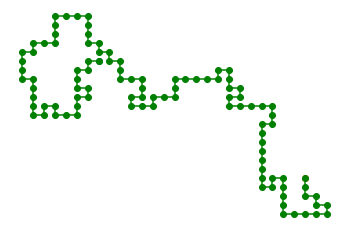
\includegraphics[width=0.45\textwidth]{../images/loose_conf.png}
	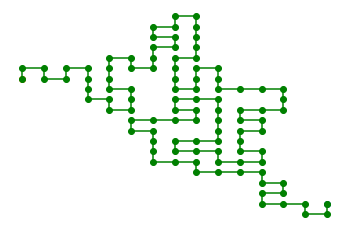
\includegraphics[width=0.45\textwidth]{../images/dense_conf.png} 
	\caption{Пример неплотной и плотной конформации}
\end{figure}

Если посмотреть на изображения конформаций каждого вида, хорошо видно, что плотные конформации по структуре близки с двумерным решёткам, где у каждого узла имеется множество соседей, и развёрнутые конформации наоборот близки к одномерным структурам, где узлы у которых больше 2 соседей встречаются редко. Соответственно можно предположить, что плотные конформации будут иметь свойства схожие с двумерными решётками, а развёрнутые с одномерными. В двумерных решётках наблюдается магнитный фазовый переход, в то время как в одномерных решётках переход не происходит. Цель данного исследования определить наличие магнитного перехода в плотных конформациях.


\subsection{Модель}
В данной модели мы рассматриваем ансамбли конформаций: множества конформаций одинаковой длинны $L$, полученные при одинаковых температурах. Мы получаем конформации используя алгоритм SAW.
На каждой из конформаций строится модель Изинга \cite{ising}. В каждой вершине размещается спин, который может принимать одно из двух значений: $+1, -1$.
Гамильтониан данной системы имеет вид
\[H = -J\sum_{\langle i, j\rangle}{\sigma_i\sigma_j} - h\sum_i{\sigma_i} \]

где $i, j$ индексы соседних узлов у, $J$- коэффициент взаимодействия $h$ - воздействие внешнего поля.

Статистическая сумма
\[Z = \sum_{\{\sigma\}} e^{-H(\sigma)\beta}, \beta = \frac{1}{kT}\]
где $\{\sigma\}$ - множество всех возможных наборов значений спинов.

Намагниченность и энергия каждого состояния считаются по следующим формулам

\[ 
E = -J\sum_{i, j} \sigma_i \sigma_j, 
M = \sum_i \sigma_i
\]

Средняя намагниченность системы

\[
\langle M \rangle = \frac{1}{Z}  \sum_{\{\sigma\}} M e^{-H_{(\sigma)}\beta}
\]

\subsection{Метод Монте-Карло}
Для расчёта модели Изинга используется метод Монте-Карло. Были реализованы версии с односпиновым и кластернным апдейтом \cite{wolf_algorithm}. Код представлен в репозитории github \cite{github}. В итоге для измерений используется кластерная версия. Благодаря отказоустойчивости она работает значительно быстрее, и быстрее сходится, особенно при низких температурах.

Алгоритм с кластерным апдейтом работает следующим образом. На каждой итерации мы выбираем случайный спин и начиная с него начинаем строить кластер из одинаково направленных спинов, добавляя новые спины в кластер с определённой вероятностью. затем мы меняем значения спинов в кластере на противоположные.

Чтобы вычислить намагниченность, мы сначала случайным образом инициализируем спины, затем делаем некоторое число шагов для отжига модели. Далее на каждом шаге мы замеряем намагниченность, и после выполнения определённого числа шагов, усредняем полученные значения. Так как средняя намагниченность равна 0, имеет смысл рассматривать модуль квадрат намагниченности.

\[
\langle M^2\rangle = \frac{1}{n} \sum_{\{\sigma\}} \left( \sum_i \sigma_i \right)^2, \\
\langle |M|\rangle = \frac{1}{n} \sum_{\{\sigma\}} \left| \sum_i \sigma_i \right|
\]